\documentclass[10pt]{article}
\usepackage[a3paper, margin=2.0cm, top=2.2cm, bottom=2.0cm]{geometry}
\usepackage{tikz}
\usetikzlibrary{arrows.meta, fit, backgrounds, calc}
\usepackage[T1]{fontenc}
\usepackage{xcolor}
\usepackage{titlesec}
\usepackage{fancyhdr}
\usepackage{booktabs}
\usepackage{amsmath}
\usepackage{amssymb}
\usepackage{parskip}
\usepackage{caption}
\usepackage{hyperref}

\definecolor{NavyD}{HTML}{0D1B2A}
\definecolor{CliD} {HTML}{1A6060}
\definecolor{CliF} {HTML}{D4EEEE}
\definecolor{MCD}  {HTML}{2C3E7A}
\definecolor{MCF}  {HTML}{DDE3F5}
\definecolor{DrmD} {HTML}{7A4010}
\definecolor{DrmF} {HTML}{FAE8D4}
\definecolor{IfcD} {HTML}{5B2080}
\definecolor{IfcF} {HTML}{EEE0FA}
\definecolor{DfiD} {HTML}{0D1F3C}
\definecolor{MGRAY}{HTML}{999999}
\definecolor{ddrblue} {HTML}{1A5276}
\definecolor{ddrgreen}{HTML}{1A7A4A}
\definecolor{ddrteal} {HTML}{0E7070}

\tikzset{
  BLK/.style args={#1/#2}{
    rectangle, rounded corners=5pt,
    draw=#1, fill=#2, text=#1,
    font=\small\bfseries, align=center,
    inner sep=6pt, minimum width=2.6cm, minimum height=1.0cm,
    line width=0.9pt
  },
  RGN/.style={draw=#1, fill=#1!5, rounded corners=8pt, dashed, line width=1.1pt},
  ARR/.style={-{Stealth[length=5pt,width=4pt]}, line width=1.0pt, color=#1},
  sbox/.style={rectangle, rounded corners=4pt, draw=#1, fill=#1!15, text=#1,
    font=\small\bfseries, align=center, inner sep=5pt, line width=0.9pt},
  ddrbox/.style={rectangle, rounded corners=3pt, draw=#1, fill=#1!20, text=#1,
    font=\scriptsize\bfseries, align=center, inner sep=4pt,
    minimum width=1.6cm, minimum height=0.5cm, line width=0.8pt},
  sarr/.style={-{Stealth[length=4pt,width=3pt]}, line width=0.85pt, color=#1},
}

\titleformat{\section}{\normalsize\bfseries\color{NavyD}}{\thesection}{0.5em}{}
  [\vspace{-3pt}\textcolor{MGRAY}{\rule{\linewidth}{0.3pt}}]
\titleformat{\subsection}{\small\bfseries\color{DfiD}}{\thesubsection}{0.5em}{}

\pagestyle{fancy}\fancyhf{}
\renewcommand{\headrulewidth}{0.3pt}
\fancyhead[L]{\scriptsize\color{MGRAY}Reconfigurable DDR Memory Controller}
\fancyhead[R]{\scriptsize\color{MGRAY}Microarchitecture Specification}
\fancyfoot[C]{\scriptsize\thepage}

\captionsetup{font=scriptsize, labelfont=bf, skip=4pt}
\hypersetup{colorlinks, linkcolor=NavyD, urlcolor=NavyD}

\begin{document}

\begin{center}
  {\Large\bfseries\color{NavyD} Reconfigurable Universal DDR Memory Controller}\\[4pt]
  {\normalsize\color{MGRAY} Microarchitecture Specification}\\[2pt]
  {\small\color{MGRAY} DDR / DDR2 / DDR3 / DDR4 / DDR5 \quad LPDDR / LPDDR2 / LPDDR3 / LPDDR4
  \quad AXI4 Host Interface \quad DFI PHY Interface}
\end{center}
\vspace{4pt}\textcolor{MGRAY}{\rule{\linewidth}{0.4pt}}\vspace{8pt}

\section{Overview}

The Reconfigurable Memory Controller (RMC) is a universal DDR
controller designed to interface with all major generations of DDR
and LPDDR SDRAM, spanning DDR through DDR5 and LPDDR through
LPDDR4, without changing the RTL. Protocol-specific behaviour
such as timing parameters and initialization sequences are loaded from a software-programmable
configuration register file at boot time.

The RMC sits between an AXI4 system interconnect and a standard
PHY interface. On the host side it accepts AXI4 burst transactions;
on the memory side it drives a DFI-compliant PHY that handles the
actual IO.

\section{System Architecture}

Figure~\ref{fig:sys} shows where the RMC sits in the full memory
subsystem. One or more AXI masters connect through a system
interconnect to the MC over AXI or CHI. The MC is the sole block
responsible for all DRAM protocol logic, translating host
transactions into correctly-timed DDR command sequences and
returning read data in order.

The MC drives a universal PHY over a standard PHY interface. The
PHY handles IO calibration, timing alignment, and differential
signaling, and fans out to whichever DDR or LPDDR generation is
physically present on the board. The scope of this document is
the MC block only.

\begin{figure}[h]
\centering
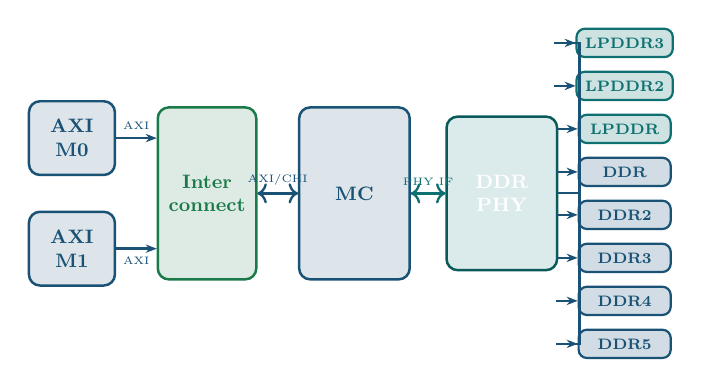
\begin{tikzpicture}[x=1cm, y=1cm, scale=0.78, every node/.style={transform shape}]
  \node[sbox=ddrblue, minimum width=1.4cm, minimum height=1.2cm] (m0) at (0, 0.9) {AXI\\M0};
  \node[sbox=ddrblue, minimum width=1.4cm, minimum height=1.2cm] (m1) at (0,-0.9) {AXI\\M1};
  \node[sbox=ddrgreen, minimum width=1.6cm, minimum height=2.8cm] (ic) at (2.2, 0) {Inter\\connect};
  \node[sbox=ddrblue, minimum width=1.8cm, minimum height=2.8cm] (mc) at (4.6, 0) {MC};
  \node[sbox=ddrteal, minimum width=1.8cm, minimum height=2.5cm,
        text=white, draw=ddrteal!80!black] (phy) at (7.0, 0) {DDR\\PHY};
  \foreach \lbl/\y/\col in {
      LPDDR3/2.45/ddrteal, LPDDR2/1.75/ddrteal, LPDDR/1.05/ddrteal,
      DDR/0.35/ddrblue, DDR2/-0.35/ddrblue, DDR3/-1.05/ddrblue,
      DDR4/-1.75/ddrblue, DDR5/-2.45/ddrblue}{
    \node[ddrbox=\col, minimum width=1.5cm, minimum height=0.46cm] (\lbl) at (9.0, \y) {\lbl};}
  \draw[sarr=ddrblue] (m0.east) -- node[above,font=\tiny]{AXI} (m0.east -| ic.west);
  \draw[sarr=ddrblue] (m1.east) -- node[below,font=\tiny]{AXI} (m1.east -| ic.west);
  \draw[sarr=ddrblue, <->] (ic.east) -- node[above,font=\tiny]{AXI/CHI} (mc.west);
  \draw[sarr=ddrteal,  <->] (mc.east) -- node[above,font=\tiny,text=ddrteal]{PHY IF} (phy.west);
  \draw[ddrblue, line width=0.8pt] (phy.east) -- ++(0.35,0) |- ($(LPDDR3.west)+(-0.35,0)$);
  \draw[ddrblue, line width=0.8pt] ($(phy.east)+(0.35,0)$) |- ($(DDR5.west)+(-0.35,0)$);
  \foreach \lbl in {LPDDR3,LPDDR2,LPDDR,DDR,DDR2,DDR3,DDR4,DDR5}{
    \draw[sarr=ddrblue] ($({\lbl}.west)+(-0.35,0)$) -- (\lbl.west);}
\end{tikzpicture}
\caption{System-level block diagram. The RMC (MC block) is the scope of this document.}
\label{fig:sys}
\end{figure}

\section{Client Domain}

The Client Domain terminates the AXI4 subordinate port and converts burst transactions
into a stream of normalized read and write commands. It has no knowledge of DRAM timing,
bank state, or refresh.

\subsection{Write Path}
An incoming AXI write burst is first split by the \textbf{Burst Splitter} if it crosses
a row or bank boundary. The \textbf{Address Translator} maps the AXI byte address to a
$\{\text{rank, bank, row, column}\}$ tuple using the mapping scheme in the register file.
The descriptor and its data are queued in the \textbf{Write Command Pool}.

\subsection{Read Path}
The read path mirrors the write path. Descriptors from the \textbf{Read Command Pool}
carry a transaction tag that the DRAM domain attaches to returning data. Completed data
passes through \textbf{Merge Logic}, which reassembles split bursts, and into the
\textbf{Reorder Buffer}, which retires responses in AXI-ID order back to the master.

\section{MC Core}

The MC Core owns the clock domain crossing. The \textbf{Async FIFO} bridges the AXI
clock (client side) and the controller clock (DRAM side), running at half the DDR data
rate. Commands cross as normalized \texttt{WR\_CMD} or \texttt{RD\_CMD} packets carrying
address, data, byte-enable mask, and transaction tag.

The \textbf{Config Registers} hold all runtime-programmable parameters: timing values,
address mapping mode, page policy, and protocol selection. The \textbf{Init FSM} steps
through the protocol-specific power-up sequence on reset, reading its command sequence
and inter-command delays from the register file, making the same FSM correct for every
supported DDR generation.

\section{DRAM Domain}

The DRAM Domain accepts commands from the internal interface and is solely responsible
for all DRAM protocol correctness.

\subsection{Scheduling Engines}
Three engines feed the central scheduler. The \textbf{Bank State Machines} track each
physical bank through Idle, Activating, Active, and Precharging states. \textbf{Timing
Control} maintains per-bank countdown timers for all JEDEC constraints ($t_{RCD}$,
$t_{RAS}$, $t_{RP}$, $t_{RFC}$, $t_{FAW}$, $t_{WTR}$, and others from the register
file) and presents an eligibility mask each cycle. The \textbf{Maintenance Engine}
handles auto-refresh, ZQ calibration, power-down entry/exit, and the post-init ready
signal.

\subsection{DDR Command Scheduler}
The scheduler selects one legal command per cycle. Priority: maintenance first (refresh
deadlines preempt everything), then row-hit reads, row-hit writes, row-miss reads, and
row-miss writes. Open-page vs.\ close-page policy is configurable per rank.

\subsection{Data Paths and DFI}
The \textbf{Write Data Path} serializes write data onto the DFI bus with correct
write-latency alignment and drives byte-mask signals. The \textbf{Read Data Path}
captures returning DFI data, associates it with the pending transaction tag, and
forwards it back to the Client Domain. All PHY commands are issued over the
\textbf{DFI Interface}; the RMC never drives DRAM pins directly.

\noindent The complete microarchitecture block diagram is on the following page.

%--- PAGE 2: MICROARCH DIAGRAM ---
\newpage
\thispagestyle{fancy}

\begin{center}
{\large\bfseries\color{NavyD} Microarchitecture Block Diagram}\\[6pt]
\end{center}

\definecolor{AW}{HTML}{1A6060}
\definecolor{AR}{HTML}{8B4500}
\definecolor{AI}{HTML}{5B2080}
\definecolor{AG}{HTML}{444444}

\centering
\begin{tikzpicture}[x=1cm,y=1cm,scale=0.65,every node/.style={transform shape}]

\node[BLK=CliD/CliF] (awp)  at (-1.7, 3.5) {AXI Write\\Port};
\node[BLK=CliD/CliF] (bsW)  at ( 1.7, 3.5) {Burst\\Splitter};
\node[BLK=CliD/CliF] (adW)  at ( 5.1, 3.5) {Address\\Translator};
\node[BLK=CliD/CliF] (wcpl) at ( 8.5, 3.5) {Write Cmd\\Pool};
\node[BLK=CliD/CliF] (arp)  at (-1.7,-3.5) {AXI Read\\Port};
\node[BLK=CliD/CliF] (bsR)  at ( 1.7,-3.5) {Burst\\Splitter};
\node[BLK=CliD/CliF] (adR)  at ( 5.1,-3.5) {Address\\Translator};
\node[BLK=CliD/CliF] (rcpl) at ( 8.5,-3.5) {Read Cmd\\Pool};
\node[BLK=CliD/CliF] (rrb)  at ( 5.1, 0.0) {Reorder\\Buffer};
\node[BLK=CliD/CliF] (mlg)  at ( 1.7, 0.0) {Merge\\Logic};

\node[BLK=IfcD/IfcF,
      minimum width=1.6cm,minimum height=9.2cm,text width=1.3cm]
  (cdc) at (12.2,0)
  {\rotatebox{90}{Async FIFO (CDC)\enspace|\enspace
    \texttt{WR\_CMD / RD\_CMD}+addr+data+tag}};

\node[BLK=MCD/MCF] (cfg)  at (15.6, 1.6) {Config\\Registers};
\node[BLK=MCD/MCF] (init) at (15.6,-1.6) {Init FSM};

\node[BLK=DrmD/DrmF] (bfsm)  at (20.1, 3.0) {Bank State\\Machines};
\node[BLK=DrmD/DrmF] (tctl)  at (20.1, 0.0) {Timing\\Control};
\node[BLK=DrmD/DrmF] (maint) at (20.1,-3.0) {Maintenance\\Engine};

\node[BLK=DrmD/DrmF,
      minimum width=3cm,minimum height=9.2cm]
  (sched) at (24.3,0) {DDR\\Command\\Scheduler};

\node[BLK=DrmD/DrmF] (wdp) at (28.1, 2.0) {Write\\Data Path};
\node[BLK=DrmD/DrmF] (rdp) at (28.1,-2.0) {Read\\Data Path};

\node[BLK=DfiD/DfiD,
      minimum width=1.6cm,minimum height=9.2cm,
      text=white,text width=1.3cm]
  (dfi) at (31.7,0)
  {\rotatebox{90}{\bfseries DFI Interface}};

\begin{scope}[on background layer]
  \node[RGN=CliD,fit=(awp)(bsW)(adW)(wcpl)(arp)(bsR)(adR)(rcpl)(rrb)(mlg),inner sep=14pt] (crgn) {};
  \node[RGN=MCD, fit=(cdc)(cfg)(init),inner sep=14pt] (mrgn) {};
  \node[RGN=DrmD,fit=(bfsm)(tctl)(maint)(sched)(wdp)(rdp)(dfi),inner sep=14pt] (drgn) {};
\end{scope}

\node[font=\large\bfseries,color=CliD,above=8pt] at (crgn.north) {Client Domain};
\node[font=\large\bfseries,color=MCD, above=8pt] at (mrgn.north) {MC Core};
\node[font=\large\bfseries,color=DrmD,above=8pt] at (drgn.north) {DRAM Domain};

\draw[ARR=AW,line width=1.3pt] (-3.2, 3.5)--(awp.west);
\draw[ARR=AR,line width=1.3pt] (-3.2,-3.5)--(arp.west);
\node[left,font=\normalsize\bfseries,color=AW] at (-3.2, 3.5) {AXI};
\node[left,font=\normalsize\bfseries,color=AR] at (-3.2,-3.5) {AXI};

\draw[ARR=AW] (awp.east)--(bsW.west);
\draw[ARR=AW] (bsW.east)--(adW.west);
\draw[ARR=AW] (adW.east)--(wcpl.west);
\draw[ARR=AR] (arp.east)--(bsR.west);
\draw[ARR=AR] (bsR.east)--(adR.west);
\draw[ARR=AR] (adR.east)--(rcpl.west);

\draw[ARR=AI] (wcpl.east)--(cdc.west|-wcpl.east);
\draw[ARR=AI] (rcpl.east)--(cdc.west|-rcpl.east);
\draw[ARR=AI] (cdc.east|-cfg)--(cfg.west);
\draw[ARR=AI] (cdc.east|-init)--(init.west);
\draw[ARR=AI,line width=1.4pt]
  (cdc.east|-tctl)--++(1,0)--++(0,0.8)--(sched.west|-{(0,0.8)});

\draw[ARR=AG,dashed,line width=0.75pt] (cfg.east)--(tctl.west);
\draw[ARR=AG,dashed,line width=0.75pt] (init.east)--(maint.west);

\draw[ARR=AG] (bfsm.east)--++(0.8,0)|-(sched.west|-bfsm.south);
\draw[ARR=AG] (tctl.east)--(sched.west);
\draw[ARR=AG] (maint.east)--++(0.8,0)|-(sched.west|-maint.north);

\draw[ARR=AW] (sched.east|-wdp)--(wdp.west);
\draw[ARR=AR] (sched.east|-rdp)--(rdp.west);

\draw[ARR=AW] (wdp.east)--++(0.8,0)|-(dfi.west|-wdp.north);
\node[above,font=\small\bfseries,color=AW] at ($(wdp.east)!0.5!(dfi.west)$){write};
\draw[ARR=AR] (dfi.west|-rdp.center)--(rdp.east);
\node[below,font=\small\bfseries,color=AR] at ($(dfi.west)!0.5!(rdp.east)$){read};

\draw[ARR=AR]
  (rdp.south) -- (rdp.south |- 0,-5.6)
  -- (rrb.south |- 0,-5.6) -- (rrb.south);
\draw[ARR=AR] (rrb.west)--(mlg.east);
\draw[ARR=AR] (mlg.west) -- ++(-4.0,0) -- ++(0,-3.5) -- (arp.west);

\draw[ARR=AG,line width=1.5pt]
  (dfi.east)--++(1,0)
  node[right,font=\normalsize\bfseries,color=DfiD]{DDR PHY};

\end{tikzpicture}

\vspace{8pt}
{\small\textbf{Figure 2:} Full microarchitecture block diagram of the RMC.
\textcolor{CliD}{\textbf{Teal}}: Client Domain;
\textcolor{MCD}{\textbf{Blue}}: MC Core;
\textcolor{DrmD}{\textbf{Amber}}: DRAM Domain.
The CDC bar is the sole crossing point between the two clock domains.}

\end{document}